\section{Dilution under controlled repetition}
\label{sec:e1}

% DRAFT 1 (2026-10-20). Only the leave-one-out subsection is written.
% Sources: results/E1_report.md (sections 3, 4.1-4.6), results/e1/<model>_summary.csv and
% <model>_beta.csv. R3D-18 with deletion: e1_metrics.py attr on the first 120 videos (same
% videos as the freezing run); all 345 videos reported in the text.

\todo{Opening paragraph: what this experiment tests (Section~\ref{sec:adding}), the number of videos and targets per model, and the share of target--control pairs that pass the gate.}

\todo{Subsection: the model's own change ($r_I$ per model; MC3-18 is the model whose dependence grows with the number of copies).}

\subsection{Overview}
\label{sec:e1-overview}

Figure~\ref{fig:bias-map} shows, for every attribution method on every model, the change in the score of one copy of the target divided by the model's own change, $r_\phi / r_I$.
An attribution that meets the requirement of Section~\ref{sec:attr-requirements} sits at 1, and an attribution that dilutes sits below 1.

\begin{figure}[t]
\centering
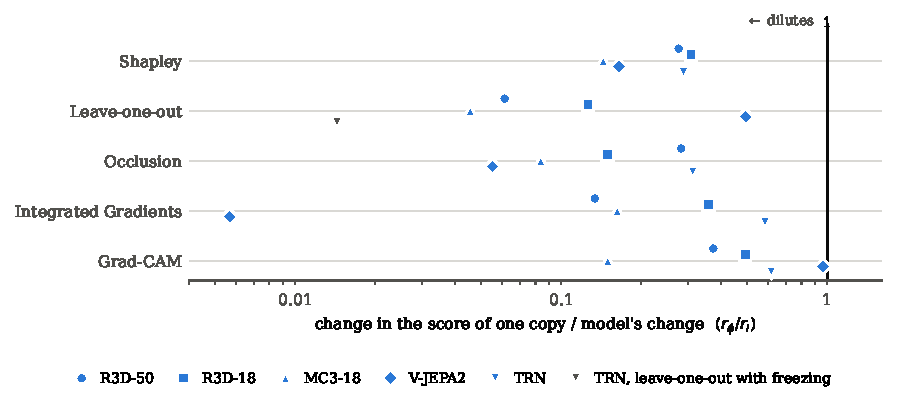
\includegraphics[width=0.85\textwidth]{figures/fig_dilution.pdf}
\caption{How much each attribution method dilutes a repeated frame, under controlled repetition (E1). The change in the score of one copy of the target divided by the model's own change, $r_\phi / r_I$, per target, then the median over targets; 1 means that the score follows the model. Largest number of copies tested (four times the reference on R3D-50 and R3D-18, nine times on MC3-18 and V-JEPA2, two times on TRN); exact copies. Leave-one-out uses deletion except on TRN (grey), where only freezing is possible and part of the result is fixed by the operator (Section~\ref{sec:removal}).}
\label{fig:bias-map}
\end{figure}

Every attribution method dilutes on every model: no point reaches 1.
How much it dilutes depends on the method and the model.
\begin{itemize}
  \item \textbf{Shapley values} keep 0.14--0.31 of the model's change per copy, on all five models.
  \item \textbf{Leave-one-out} keeps 0.05--0.49 with deletion, and 0.01 on TRN with freezing. \textbf{Occlusion} keeps 0.06--0.31.
  \item \textbf{Integrated Gradients} varies most between models: from 0.006 on V-JEPA2 to 0.58 on TRN.
  \item \textbf{Grad-CAM} comes closest to the model, at 0.37--0.96 on four models. On MC3-18, whose dependence on the target triples, it keeps 0.15.
\end{itemize}
These values are medians of per-target ratios, so they differ from the medians of the per-copy scores reported in Table~\ref{tab:e1-loo} and in the E1 report, which are taken separately from the median of $r_I$.
% Source: motivation/fig_dilution.py (prints every plotted value).

\todo{Subsection: Shapley values and Play Fair.}

\subsection{Leave-one-out}
\label{sec:e1-loo}

Leave-one-out depends on the removal operator, and with freezing part of its result is fixed by the operator alone (Section~\ref{sec:why}, Appendix~\ref{app:loo-freeze}).
We therefore report it with deletion wherever the model allows it: on MC3-18 and V-JEPA2, which use deletion throughout, and on R3D-50 and R3D-18, where removing a single frame shortens the clip only from 16 to 15 frames (Section~\ref{sec:removal}).
TRN accepts only 8 frames, so for TRN we can only report leave-one-out with freezing.
Table~\ref{tab:e1-loo} gives both operators for the R3D models, to show how much the operator matters.

\begin{table}[h]
\centering
\caption{Leave-one-out under controlled repetition, at the largest number of copies tested. ``Copies'' is the number of copies of the target relative to the reference clip. $r_I$ is the model's own change in dependence on the target. Score per copy: the mean leave-one-out score of one copy of the target, relative to the reference clip, for the target clip and for the control clip. $\beta$: dilution slope with 95\% bootstrap interval ($\beta = -1$ is an even split among the copies). Medians over targets. Exact copies. Freezing rows for TRN, and for R3D-50 and R3D-18 for comparison, are marked $^\dagger$: their scores are partly fixed by the operator.}
\label{tab:e1-loo}
\begin{tabular}{llccccc}
\toprule
 & & & & \multicolumn{2}{c}{score per copy} & \\
\cmidrule(lr){5-6}
model & removal & copies & $r_I$ & target & control & $\beta$, target (control) \\
\midrule
R3D-50  & deletion & $\times 4$ & 1.28 & 0.01 & 0.64 & $-0.27$ $[-0.72, -0.15]$ ($+0.17$) \\
R3D-18  & deletion & $\times 4$ & 1.30 & 0.36 & 0.56 & $\phantom{-}0.00$ $[-0.26, \phantom{-}0.17]$ ($+0.13$) \\
MC3-18  & deletion & $\times 9$ & 3.22 & 0.13 & 0.70 & $-0.77$ $[-0.84, -0.70]$ ($-0.14$) \\
V-JEPA2 & deletion & $\times 9$ & 0.87 & 0.30 & 0.83 & $-0.48$ $[-0.69, -0.22]$ ($-0.05$) \\
\midrule
TRN     & freezing$^\dagger$ & $\times 2$ & 1.32 & 0.02 & 1.03 & $-2.60$ $[-3.19, -2.25]$ ($+0.25$) \\
R3D-50  & freezing$^\dagger$ & $\times 4$ & 1.28 & $-0.05$ & 0.39 & $-1.38$ $[-1.91, -1.07]$ ($-0.11$) \\
R3D-18  & freezing$^\dagger$ & $\times 4$ & 1.30 & $-0.02$ & 0.62 & $-1.55$ $[-1.69, -1.38]$ ($-0.09$) \\
\bottomrule
\end{tabular}
\end{table}

\paragraph{With deletion, leave-one-out dilutes on every model where it can be tested.}
On all four models, the score of one copy of the target falls well below its value in the control clip, and well below the model's own change in dependence on the target ($r_I$ between 0.87 and 3.22).
How far it falls depends on the model.
On R3D-50, each copy keeps almost none of its score (0.01).
On MC3-18, it keeps 0.13, although the model's dependence on the target more than triples.
On V-JEPA2 and R3D-18, it keeps 0.30 and 0.36.
On R3D-18, 0.36 is close to an even split of the model's dependence among four times as many copies ($1.30 / 4 = 0.33$).
The dilution slope of the target lies clearly below that of its control on MC3-18 and V-JEPA2, where the two intervals do not overlap.
On R3D-50 it is also below, but the interval of the control ($[-0.18, +0.43]$) overlaps that of the target slightly.
On R3D-18, the two intervals overlap on the 120 videos used for the comparison with freezing; on all 345 videos with E1 clips, the slope is $-0.19$ $[-0.31, -0.08]$ for the target and $+0.08$ $[+0.02, +0.18]$ for the control, with 0.44 per copy.

\paragraph{With freezing, the score per copy is close to zero on every model, but this is partly fixed by the operator.}
On R3D-50, deletion gives a similar result (0.01 against $-0.05$ per copy), so there the near-zero score does not come from the operator.
On R3D-18, it does: deletion gives 0.36 per copy and a slope of 0.00, against $-0.02$ and $-1.55$ with freezing.
On TRN, we cannot separate the two.
Its result is consistent with dilution, but part of it may come from the operator, as on R3D-18.

\todo{Subsection: occlusion, Integrated Gradients and Grad-CAM (score per copy, against the model's change and against the control clips).}

\todo{Subsection: rankings (inversions; leave-one-out with deletion on R3D-18: 50\% against 37\% in the control).}
